\begin{figure}[H]
    \centering
    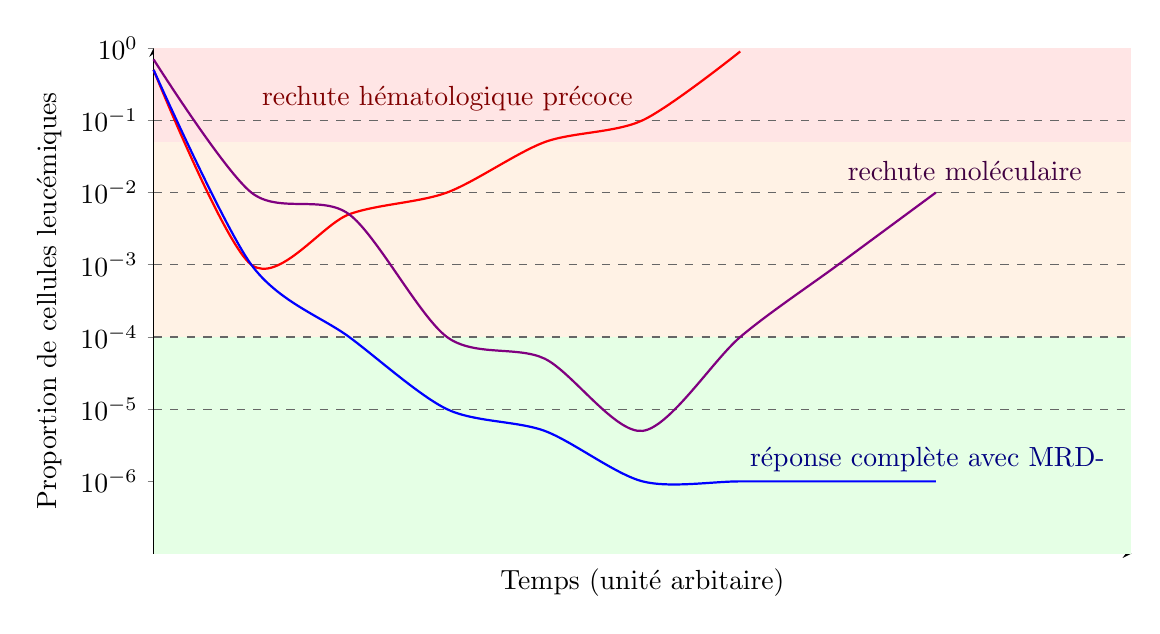
\begin{tikzpicture}
    \begin{semilogyaxis}[
        width=14cm,
        height=8cm,
        xlabel={Temps (unité arbitaire)},
        ylabel={Proportion de cellules leucémiques},
        ymin=1e-7, ymax=1,
        ytick={1e0,1e-1,1e-2,1e-3,1e-4,1e-5,1e-6},
        yticklabels={$10^{0}$,$10^{-1}$,$10^{-2}$,$10^{-3}$,$10^{-4}$,$10^{-5}$,$10^{-6}$},
        xtick=\empty,
        axis lines=left,
        grid=none,
        clip=false,
    ]

    % sections d'arrière plan
    \addplot [draw=none, fill=red!10]
     coordinates {
        (0,1e0) (10,1e0) (10,5e-2) (0,5e-2)
    } -- cycle;

    \addplot [draw=none, fill=orange!10
    ] coordinates {
        (0,5e-2) (10,5e-2) (10,1e-4) (0,1e-4)
    } -- cycle;

    \addplot [draw=none, fill=green!10
    ] coordinates {
        (0,1e-4) (10,1e-4) (10,1e-7) (0,1e-7)
    } -- cycle;

    % lignes horizontales pour les seuils
    \foreach \y in {1e-1,1e-2,1e-3,1e-4,1e-5} {
        \addplot[dashed, color=black!60] coordinates {(0,\y) (10,\y)};
    }

    % réponse complète avec MRD-
    \addplot[thick, red, smooth] coordinates {
        (0,5e-1) (1,1e-3) (2,5e-3) (3,1e-2) (4,5e-2) (5,1e-1) (6,9e-1)
    };

    % rechute précoce
    \addplot[thick, blue, smooth] coordinates {
        (0,5e-1) (1,1e-3) (2,1e-4) (3,1e-5) (4,5e-6) (5,1e-6) (6,1e-6) (7,1e-6) (8,1e-6)
    };

    % rechute moléculaire 
    \addplot[thick, violet, smooth] coordinates {
        (0,7e-1) (1,1e-2) (2,5e-3) (3,1e-4) (4,5e-5) (5,5e-6) (6,1e-4) (7,1e-3) (8,1e-2)
    };

    % labels
    \node[align=left, anchor=west, blue!50!black] at (axis cs:6,2e-6) {réponse complète avec MRD-};
    \node[align=left, anchor=west, violet!50!black] at (axis cs:7,2e-2) {rechute moléculaire};
    \node[align=center, anchor=south east, red!50!black] at (axis cs:5,1e-1) {rechute hématologique précoce};

    \end{semilogyaxis}
    \end{tikzpicture}
    \caption{Suivi de la \gls{mrd} dans le temps. Exemple de trois réponses différentes selon le statut 
    de la \gls{mrd} : \textcolor{blue}{réponse complète avec \gls{mrd}- en blue},  
    \textcolor{red}{rechute précoce en rouge} et \textcolor{violet}{rechute moléculaire en violet}.}
    \label{fig:mrd}
\end{figure}
